\tikzset{every picture/.style={line width=0.75pt}} %set default line width to 0.75pt        

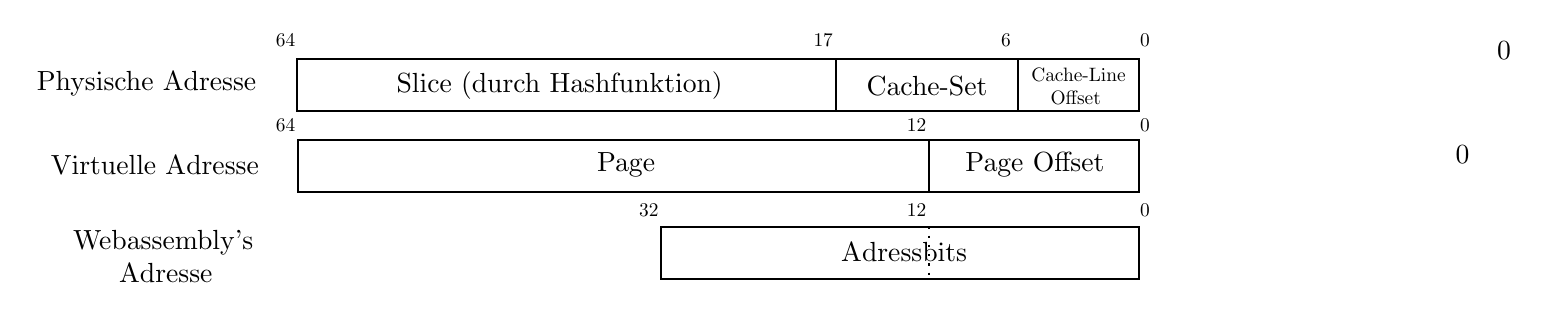
\begin{tikzpicture}[x=0.75pt,y=0.75pt,yscale=-1,xscale=1]
%uncomment if require: \path (0,147); %set diagram left start at 0, and has height of 147

%Shape: Rectangle [id:dp378127113165748] 
\draw   (139.4,25) -- (399,25) -- (399,50) -- (139.4,50) -- cycle ;
%Shape: Rectangle [id:dp46142039984044336] 
\draw   (139.8,64) -- (444,64) -- (444,89) -- (139.8,89) -- cycle ;
%Shape: Rectangle [id:dp8338046143479867] 
\draw   (399,25) -- (487,25) -- (487,50) -- (399,50) -- cycle ;
%Shape: Rectangle [id:dp940182630841411] 
\draw   (487,25) -- (545,25) -- (545,50) -- (487,50) -- cycle ;
%Shape: Rectangle [id:dp12367960229267094] 
\draw   (444,64) -- (545,64) -- (545,89) -- (444,89) -- cycle ;
%Shape: Rectangle [id:dp7768353739474505] 
\draw   (315,106) -- (545.33,106) -- (545.33,131) -- (315,131) -- cycle ;
%Straight Lines [id:da18312510628843603] 
\draw  [dash pattern={on 0.84pt off 2.51pt}]  (443.9,105.6) -- (443.9,129.6) ;

% Text Node
\draw (721,21) node   {$0$};
% Text Node
\draw (701,71) node   {$0$};
% Text Node
\draw (67,37) node  [align=left] {Physische Adresse};
% Text Node
\draw (71,76) node  [align=left] {Virtuelle Adresse};
% Text Node
\draw (75,120) node  [align=left] {Webassembly's\\ \ \ \ \ \ Adresse};
% Text Node
\draw (516,38) node [scale=0.7] [align=left] {Cache-Line\\ \ \ \ Offset};
% Text Node
\draw (443,38) node [scale=1] [align=left] {Cache-Set};
% Text Node
\draw (266,38) node [scale=1] [align=left] {Slice (durch Hashfunktion)};
% Text Node
\draw (134,16) node [scale=0.7] [align=left] {64};
% Text Node
\draw (393,16) node [scale=0.7] [align=left] {17};
% Text Node
\draw (481,16) node [scale=0.7] [align=left] {6};
% Text Node
\draw (548,16) node [scale=0.7] [align=left] {0};
% Text Node
\draw (298,76) node [scale=1] [align=left] {Page};
% Text Node
\draw (495,76) node [scale=1] [align=left] {Page Offset};
% Text Node
\draw (438,57) node [scale=0.7] [align=left] {12};
% Text Node
\draw (309,98) node [scale=0.7] [align=left] {32};
% Text Node
\draw (548,57) node [scale=0.7] [align=left] {0};
% Text Node
\draw (548,98) node [scale=0.7] [align=left] {0};
% Text Node
\draw (438,98) node [scale=0.7] [align=left] {12};
\draw (134,57) node [scale=0.7] [align=left] {64};
% Text Node
\draw (432,118) node [scale=1] [align=left] {Adressbits};

\end{tikzpicture}